\documentclass[11pt]{article}
\usepackage[utf8]{inputenc}
\usepackage{amsmath, amssymb}
\usepackage{graphicx}
\usepackage{hyperref}
\usepackage{geometry}
\usepackage[backend=biber]{biblatex}
\addbibresource{../references.bib}
\geometry{margin=1in}

\title{The Abstract Universe Project: Technical Introduction}
\author{Abstract Author}
\date{\today}

\begin{document}

\maketitle

\section{Introduction}

This paper presents the foundational framework of the Abstract Universe Project — a radically minimalistic approach to a theory of everything, grounded purely in information theory. The core idea is that all physical reality, including conscious observers, spacetime, and matter, can be derived from finite binary strings and their compressions. By applying principles of computational theory, wavefunction superposition, and observer-centric reasoning, the theory posits that familiar physics — including gravity and quantum mechanics — emerges from entropy gradients in bitstrings and their probabilistic arrangements. The observer, rather than being external, is modeled as a substring within a finite universe, offering a self-contained, emergent, and minimal framework.

The theory builds on two foundational unpublished manuscripts \cite{meskanen2019, meskanen2020}.

\section{The Observational Assumptions}

The theory is based on the following observational assumptions \cite{meskanen2019}:

\begin{itemize}
      \item \textbf{Assumption 1:} DNA Contains Sufficient Information for Consciousness.
      \item \textbf{Assumption 2:} DNA Obeys Physical Laws.
      \item \textbf{Assumption 3:} The Church–Turing Thesis Holds.
      \item \textbf{Assumption 4:} Pain Has Measurable Physical Effects.
\end{itemize}

The fourth assumption is essential for bringing consciousness out of the realm of purely philosophical or subjective discourse and into the domain of physics.

\[
      \text{Human} + \text{Pain} \neq \text{Human}
\]

If a human experiencing pain behaves differently from one who does not, then pain produces measurable effects. In this sense, pain becomes analogous to a physical force—its presence alters observable outcomes. This reasoning extends to other subjective experiences, including consciousness: if an experience systematically correlates with measurable behavior, it becomes accessible to scientific investigation and, thus, part of physics.

If these assumptions hold, it follows that information and its structured arrangements alone can explain the universe as we observe it.

\section{Information}

We do not fully understand what information is at its core. Similarly, the fundamental nature of human consciousness remains elusive.

However, assuming the four observational assumptions hold, everything within human consciousness can, in principle, be duplicated using a Turing machine or its modern counterpart—a computer. From this, we derive:

\begin{itemize}
      \item Computers are based on binary systems, whose operations are formally understood.
      \item Set theory is sufficient to describe the structure of binary computation.
\end{itemize}

\textbf{Conclusion:} Binary systems—bits—are a sufficient and complete informational foundation to describe reality.

Since set-theoretical descriptions can be lengthy, we use the term "bitstring" as a synonym for an ordered set of binary elements.

\section{Definition of Reality}

We define \textbf{reality} as the set of observable phenomena that can, in principle, be measured and whose outcomes can be compared to predictions made by a scientific theory. This definition aligns with the scientific method.

\section{Universe with Observer in It}

We observe a vast universe \( U \) that includes ourselves. To model this, we define:

\[
      O \subseteq U
\]

We also observe time as a unidirectional flow, advancing continuously and carrying us through the evolving universe:

\[
      \forall t_1, t_2 \in T,\quad t_2 > t_1 \Rightarrow t_2 \text{ is in the future of } t_1
\]

\section{Philosophical Elegance — Mathematical Minimalism}

The Abstract Universe Project seeks to derive all of physics from the four basic assumptions. The only philosophical principle introduced is the requirement that the theory be free of any predefined substrate. It must be self-contained, with all physical laws arising as emergent properties rather than as assumed primitives.

From this perspective, we critique existing physical theories. General Relativity assumes the existence of spacetime without explaining its origin. It relies on experimentally determined constants—such as the gravitational constant \(G\), the speed of light \(c\), and the cosmological constant \(\Lambda\)—which it does not explain.

Similarly, the Standard Model of quantum mechanics depends on at least 19 empirical constants, whose values are not derived within the theory. This reliance undermines its self-contained explanatory power.

\section{The Abstract Universe Project}

We use bits as the elementary building blocks of the universe. The universe \(U\) is modeled as a finite bitstring. The observer \(O\) is modeled as a substring within \(U\).

\subsection{Information-Theoretic Probability of Consciousness}

As shown in \cite{meskanen2019}, a bitstring of pure noise, given sufficient length, will eventually describe a conscious observer. The information in \(n\) bits can be arranged in \(2^n\) ways.

Let \(O \subseteq U\) be an observer embedded within the universe. Suppose the internal informational state of the observer is encoded by a bitstring of length \(n\). Then the number of possible configurations is:

\[
      |\mathcal{C}| = 2^n
\]

Let \(\mathcal{C}_{\text{conscious}} \subseteq \mathcal{C}\) be the subset corresponding to coherent, intelligent, and conscious observers. Then the probability of consciousness is:

\[
      P_{\text{conscious}} = \frac{|\mathcal{C}_{\text{conscious}}|}{2^n}
\]

This quantifies how rare or typical conscious arrangements are within the space of all informational configurations.

\subsection{The Problem with Memory}

For an observer to remember or perceive anything, their bitstring must contain information reflecting the external universe. Since the system is entirely self-contained, no external signals transmit information. Thus, any knowledge the observer has must already be embedded in the bitstring.

\begin{figure}[h!]
      \centering
      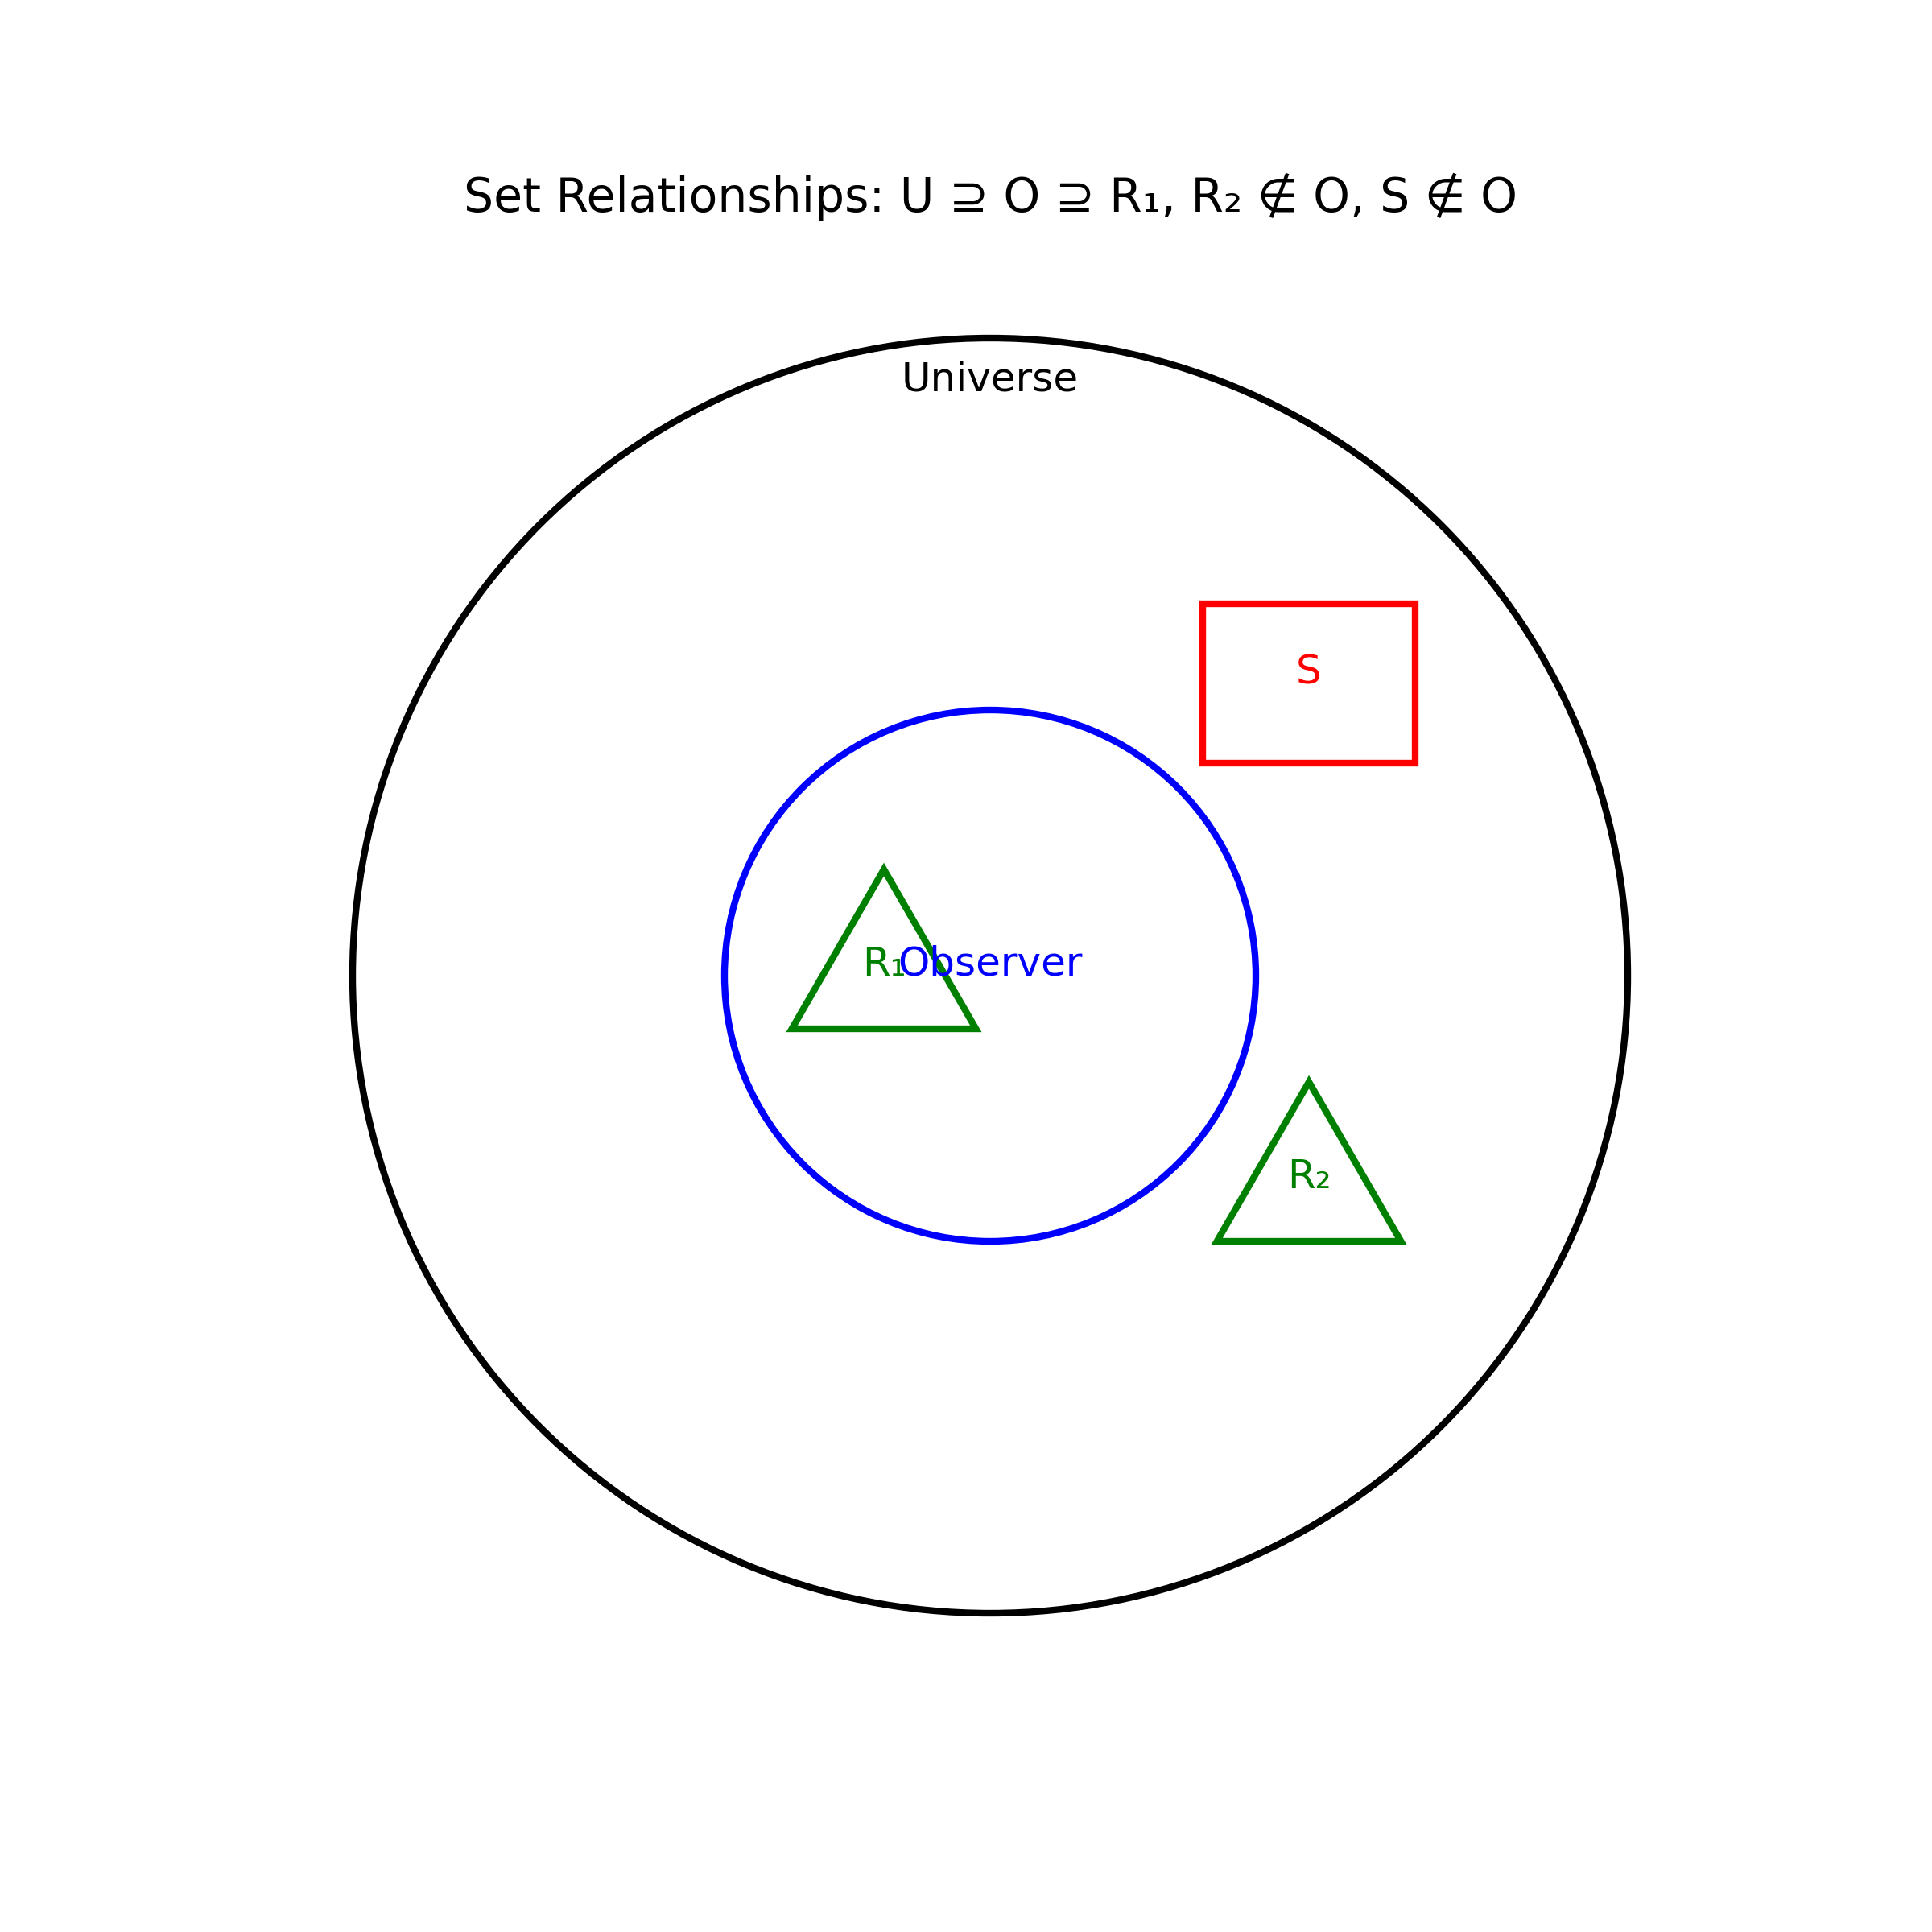
\includegraphics[width=1.0\textwidth]{figures/memory.png}
      \caption{An observer with embedded knowledge about the surrounding universe.}
      \label{fig:memory}
\end{figure}

Observers are most likely to find themselves in bitstrings that contain both a coherent sense of self and a structured surrounding universe. Continuity of experience requires:

\[
      \mathrm{Sim}(\psi_t, \psi_{t+1}) \geq \epsilon
\]

for some \(\epsilon > 0\), ensuring the observer retains memory and identity.

\subsection{The Nature of the Wavefunction}

Despite the observationally verified randomness in quantum mechanics, the wavefunction is deterministic and defines probabilistic outcomes. We argue this duality has a logical basis.

\subsection{The Wavefunction as a Compression Algorithm}

We assume:

\begin{itemize}
      \item The observer-centric principle: the observer only exists in universes that encode them.
      \item Universes that describe more observers are more probable.
\end{itemize}

\textbf{Conclusion:} The wavefunction is a compression algorithm for describing a conscious observer using a minimal number of bits. The sine wave, being the simplest periodic function, emerges naturally and leads to quantum mechanics.

\subsection{Binary Representations of Reality}

We model reality as finite-length binary strings:

\[
      b \in \{0,1\}^n
\]

\subsection{Observers as Substrings}

An observer is defined by a subset of bit positions:

\[
      P \subseteq \{0, \dots, n-1\}
\]

with observed data:

\[
      O = b|_P
\]

This defines the observer as a projection of the universal bitstring.

\subsection{Wavefunction Representation}

Though the wavefunction is continuous in traditional quantum mechanics, we propose that it is actually a discrete structure that only appears smooth due to the universe’s large informational content.

We assume the bitstring includes both data and algorithm. The observer is defined by this algorithm—a sum of frequencies and phases. Formally, we write:

\[
      \psi \in \mathbb{C}^d,\quad \|\psi\| = 1
\]

\subsection{Duality of Bitstrings and Wavefunctions}

\begin{itemize}
      \item \textbf{Bitstrings} provide the concrete informational substrate.
      \item \textbf{Wavefunctions} are optimal, compressed, and predictive models of that substrate.
\end{itemize}

This duality allows both discrete and continuous descriptions.

\section{Subjective Time and Wavefunction Evolution}

\subsection*{The Observer Inside a Pure-State Universe}

Following Everett \cite{everett1957relative}, Hartle and Hawking \cite{hartle1983wave}, and others \cite{maldacena1998largeN, witten1998ads, rovelli1997loop}, we model the universe as a pure wavefunction \(|\Psi\rangle\) in Hilbert space \(\mathcal{H}_U\).

We define:

\[
      \mathcal{H}_U = \mathcal{H}_O \otimes \mathcal{H}_R
\]

The observer's reduced state is:

\[
      \rho_O = \mathrm{Tr}_R \left( |\Psi\rangle \langle \Psi| \right)
\]

If the universal state is entangled, then \(\rho_O\) is mixed, and reality appears probabilistic.

\subsection*{Time as Ensemble Indexing}

We define time as a sequence of informational states:

\[
      T = \{ \psi_0, \psi_1, \psi_2, \ldots \}
\]

Each \(\psi_t\) encodes the observer’s state at time \(t\).

\subsection*{Unitary Evolution}

Evolution is modeled as:

\[
      \psi_{t+1} = U \psi_t
\]

where \(U\) preserves continuity and maximizes internal compressibility.

\section{Compression, Superposition, and Emergent Physics}

\subsection{Compression as a Selection Principle}

We favor universes with minimal algorithmic complexity:

\[
      \min_U C(U)
\]

\subsection{Wavefunction Superposition}

The wavefunction encodes possible futures:

\[
      \psi = \sum_i c_i \phi_i
\]

Interference arises from overlapping structure, producing quantum phenomena.

\subsection{Emergent Geometry and Dynamics}

Spacetime geometry, locality, and causality emerge from patterns in the wavefunction. Increasing entropy corresponds to increasing structural complexity, which manifests as expanding spacetime.

Gravity arises from probability distributions over arrangements. Observers fall because those configurations are statistically dominant in compressed representations.

\section{Discussion and Outlook}

This framework makes several predictions:

The wavefunction has discrete structure.

\[TODO\]

It predicts perfectly smooth, zero-entropy initial state and an entropy-driven expansion.

The observer’s wavefunction evolves through compressive selection, supporting consistent conscious trajectories.

\section {Future Work}

Future work will explore how General Relativity can be understood as an emergent description arising from the probability distribution of the observer’s states within the spacetime manifold.

Include simulations illustrating entropy–geometry correspondence and exploring empirical implications of the model.

Implement two-slit experiment as python script.

\printbibliography

\end{document}
